\documentclass{beamer}

\title{Introduction to mechanistic ecological niche models}
\subtitle{Day 1: Introduction}
\date{2026-06-08}

% Options for packages loaded elsewhere
\PassOptionsToPackage{unicode=true}{hyperref}
\PassOptionsToPackage{hyphens}{url}
\PassOptionsToPackage{dvipsnames,svgnames,x11names}{xcolor}

% ---------- Packages ----------
\usepackage{booktabs}
\usepackage{array}
\usepackage[absolute,overlay]{textpos}
\usepackage{pgfpages}
\usepackage{minted}
\definecolor{mintedbg}{rgb}{0.969,0.969,0.969}
\setminted{
  bgcolor=mintedbg,
  fontsize=\tiny,
  breaklines=true,
  tabsize=2,
  style=tango,
}
\usepackage{tikz}
\usetikzlibrary{shapes.callouts, shapes.arrows, arrows.meta, calc, positioning}
\usetikzlibrary{decorations.pathmorphing}
\usetikzlibrary{backgrounds}
\usepackage{mathtools}
% \usepackage[thinc]{esdiff}
\usepackage{physics}
\usepackage{graphicx}
\usepackage[dvipsnames]{xcolor}
\usepackage{fontawesome}
\usepackage{csquotes}
\usepackage{bookmark}
\usepackage[font=tiny]{caption}

% ---------- Beamer configuration ----------
\usetheme{Triton}
\setbeamertemplate{caption}[numbered]
\setbeamertemplate{caption label separator}{: }
\setbeamercolor{caption name}{fg=normal text.fg}
\beamertemplatenavigationsymbolsempty

% Prevent slide breaks in the middle of a paragraph
\widowpenalties 1 10000
\raggedbottom

% Section pages
\setbeamertemplate{section page}{
  \centering
  \begin{beamercolorbox}[sep=12pt,center]{part title}
    \usebeamerfont{section title}\insertsection\par
  \end{beamercolorbox}
}

% Fonts
\usefonttheme[onlymath]{serif}
\usepackage{lmodern}

% Graphics setup
\makeatletter
\def\maxwidth{\ifdim\Gin@nat@width>\linewidth\linewidth\else\Gin@nat@width\fi}
\def\maxheight{\ifdim\Gin@nat@height>\textheight\textheight\else\Gin@nat@height\fi}
\makeatother
\setkeys{Gin}{width=\maxwidth,height=\maxheight,keepaspectratio}
\makeatletter
\def\fps@figure{htbp}
\makeatother

% ---------- Biblatex ----------
\usepackage[backend=biber,style=apa]{biblatex}
\addbibresource{/home/urtzi/Documents/zotero.bib}

% ---------- Hyperref ----------
\usepackage{hyperref}
\hypersetup{
  colorlinks=true,
  linkcolor=Blue,
  filecolor=Blue,
  citecolor=Blue,
  urlcolor=Blue,
  pdfcreator={LaTeX via knitr}
}
\urlstyle{same}


% ---------- Author ----------
\author{Urtzi Enriquez-Urzelai\inst{1}}

% ---------- Institute ----------
\institute{
  \inst{1} Institute of Vertebrate Biology, \\
  Czech Academy of Sciences
  \newline \newline
  \faGithub \hspace*{0.2ex}
  \href{https://github.com/urtzienriquez}{\color{blue}{GitHub}}
  \hspace*{0.5ex}
  \faGlobe \hspace*{0.2ex}
  \href{https://urtzienriquez.github.io/}{\color{blue}{webpage}}
}

% ---------- Title graphic ----------
\titlegraphic{
  \begin{minipage}[b]{0.20\textwidth}
    \raggedright
    ~
  \end{minipage}%
  \begin{minipage}[b]{0.20\textwidth}
    \raggedright
    ~
  \end{minipage}%
  \begin{minipage}[b]{0.20\textwidth}
    \centering
    
\includegraphics[height=1cm]{/home/urtzi/Documents/courses/usfq_mnm/resources/images/ivb-logo.png}
  \end{minipage}%
  \begin{minipage}[b]{0.20\textwidth}
    \raggedright
    ~
  \end{minipage}%
  \begin{minipage}[b]{0.20\textwidth}
    \raggedright
    \tiny Organized by: \\ [0.5ex]
    
\includegraphics[height=0.6cm]{/home/urtzi/Documents/courses/usfq_mnm/resources/images/usfq-logo.png}
  \end{minipage}
}
\usepackage{xcolor}
\usepackage{minted}
\definecolor{knitbg}{rgb}{0.969, 0.969, 0.969}
\usepackage{graphicx}
\makeatletter
\def\maxwidth{ %
  \ifdim\Gin@nat@width>\linewidth
    \linewidth
  \else
    \Gin@nat@width
  \fi
}
\makeatother

\begin{document}




\frame{\titlepage}

\begin{frame}
  \frametitle{Disecting\ldots}
  \Large
  \centering
  \textcolor<1-2>{gray!25}{mechanistic}
  \textcolor<1>{gray!25}{ecological niche}
  \textcolor<1-2>{gray!25}{models}
\end{frame}

\section{Niches}

\begin{frame}
  \frametitle{What is the ecological niche?}
  \setbeamercovered{transparent=20}
  \begin{columns}[c]
    \column{0.45\textwidth}
    \small
    \uncover<1-1>{
      \textbf{Grinnell (1917)} \nocite{grinnell1917}
      \begin{itemize}
        \item niche as climatic and habitat requirements
        \item emphasis on abiotic conditions
      \end{itemize}
      \vspace{0.2cm}
    }
    \uncover<2->{
      \textbf{Elton (1927)} \nocite{elton1927}
      \begin{itemize}
        \item niche as the role of a species
        \item emphasis on biotic interactions
      \end{itemize}
    }
    \column{0.5\textwidth}
    \begin{overlayarea}{\textwidth}{0.7\textheight}
      \only<1>{
        \begin{figure}
          \begin{tikzpicture}
            \node (g_picture) {
              
\includegraphics[width=0.4\textwidth]{/home/urtzi/Documents/courses/usfq_mnm/resources/images/grinnell.png}
            };
            \node[anchor=north] at (g_picture.south) (g_book) {
              
\includegraphics[width=\textwidth]{/home/urtzi/Documents/courses/usfq_mnm/resources/images/grinnell_book.png}
            };
          \end{tikzpicture}
        \end{figure}
      }
      \only<2>{
        \begin{figure}
          \begin{tikzpicture}
            \node (e_picture) {
              
\includegraphics[width=0.4\textwidth]{/home/urtzi/Documents/courses/usfq_mnm/resources/images/elton.jpg}
            };
          \end{tikzpicture}
        \end{figure}
      }
    \end{overlayarea}
  \end{columns}
\end{frame}

\begin{frame}
  \frametitle{Hutchinson's take}

  \vspace{0.2cm}

  \textbf{Hutchinson (1957)} \nocite{hutchinson1957}
  \begin{itemize}
    \item niche as an \textbf{n-dimensional hypervolume}
    \item defined in environmental space
    \item conditions allowing population persistence
  \end{itemize}

  \vspace{1cm}

  \begin{quote}
    \scriptsize
    \raggedleft
    "The niche is defined as an n-dimensional hypervolume"

    \textbf{--- Hutchinson (1957)}
  \end{quote}

\end{frame}

\begin{frame}
  \frametitle{BAM diagram}

  \vspace{1cm}
  \centering
  \begin{figure}
    \begin{tikzpicture}[
        a/.style={fill, fill opacity=0.1},
        bubble/.style={
            draw,
            overlay,
            fill=yellow!40,
            rounded corners,
            align=flush center,
            rectangle callout,
            font=\scriptsize,
            inner sep=5pt
          },
        scale=0.8,
      ]
      \def\Acircle{(2.3,3.7) circle (1.5)}
      \def\Bcircle{(3.7,3.7) circle (1.5)}
      \def\Mcircle{(3,2.2) circle (1.5)}
      \def\Grectangle{(0,0) rectangle (6,6)}
      \uncover<1->{
        \draw \Grectangle;
        \node[inner sep=0] at (0.5,5.5) (labelG) {G};
      }
      \uncover<2->{
        \filldraw[a,green] \Acircle;
        \node[inner sep=0] at (1.5,4.5) (labelA) {A};
      }
      \uncover<3->{
        \filldraw[a,blue] \Bcircle;
        \node[inner sep=0] at (4.5,4.5) (labelB) {B};
      }
      \uncover<4->{
        \filldraw[a,red] \Mcircle;
        \node[inner sep=0] at (3,1.2) (labelM) {M};
      }
      \uncover<5>{
        \begin{scope}
          \clip \Acircle;
          \clip \Bcircle;
          \fill[gray,opacity=0.6] \Grectangle;
          \coordinate (centerAB) at (3, 3.67);
        \end{scope}
      }
      \uncover<6>{
        \begin{scope}
          \clip \Acircle;
          \clip \Bcircle;
          \pgfseteorule \clip \Grectangle \Mcircle;
          \fill[gray,opacity=0.6] \Grectangle;
          \coordinate (centerABnM) at (3, 4);
        \end{scope}
      }
      \uncover<7>{
        \begin{scope}
          \clip \Acircle;
          \clip \Bcircle;
          \clip \Mcircle;
          \fill[gray,opacity=0.6] \Grectangle;
          \coordinate (centerABM) at (3, 3);
        \end{scope}
      }
      \uncover<8>{
        \fill[gray,opacity=0.6] \Acircle;
      }
      \uncover<1-4>{
        \node[
          bubble,
          callout absolute pointer={(labelG.west)},
          text width=3cm
        ]
        at (-2.5,6)
        {
          \textbf{Geographical space}};
      }
      \uncover<2-4>{
        \node[
          bubble,
          callout absolute pointer={(labelA.south west)},
          text width=3cm
        ]
        at (-2.5,3)
        {
          \textbf{Abiotic conditions}\\ 
          Scenopoetic variables (e.g., temperature, relative humidity and radiation).
        };
      }
      \uncover<3-4>{
        \node[
          bubble,
          callout absolute pointer={(labelB.east)},
          text width=3cm
        ]
        at (8.5,4.5)
        {
          \textbf{Biotic conditions}\\ 
          Bionomic variables (e.g., competitors, predators and diseases).
        };
      }
      \uncover<4>{
        \node[
          bubble,
          callout absolute pointer={(labelM.east)},
          text width=3cm
        ]
        at (8.5,1)
        {
          \textbf{Movement}\\ 
          Regions accessible to the species.
        };
      }
      \uncover<5>{
        \node[bubble, callout absolute pointer={(centerAB)}, text width=2.5cm]
        at (8.5,4.5)
        {Potential distribution};
      }
      \uncover<6>{
        \node[bubble, callout absolute pointer={(centerABnM)}, text width=2.5cm]
        at (8.5,4.5)
        {Potentially invasible area};
      }
      \uncover<7>{
        \node[bubble, callout absolute pointer={(centerABM)}, text width=2.5cm]
        at (8.5,4.5)
        {Realized distribution};
      }
      \uncover<8>{
        \node[bubble, callout absolute pointer={(2.3,3.7)}, text width=2.5cm]
        at (8.5,4.5)
        {Fundamental niche/distribution};
      }
    \end{tikzpicture}
    \caption{\tiny Based on \textcite{soberon2009} and \textcite{sillero2011}.}
  \end{figure}

\end{frame}

\begin{frame}
  \frametitle{From niches to distributions}

  \vspace{1cm}
  \begin{figure}
    \begin{columns}[c]
      \begin{column}{0.45\textwidth}
        \centering
        \only<1->{
          
\includegraphics[height=0.6\textheight]{/home/urtzi/Documents/courses/usfq_mnm/resources/images/hypervolume.png}
        }
      \end{column}
      \begin{column}{0.45\textwidth}
        \centering
        \only<2>{
          
\includegraphics[height=0.6\textheight]{/home/urtzi/Documents/courses/usfq_mnm/resources/images/hypervolume_in_space1.jpg}
        }
        \only<3>{
          
\includegraphics[height=0.6\textheight]{/home/urtzi/Documents/courses/usfq_mnm/resources/images/hypervolume_in_space2.jpg}
        }
      \end{column}
    \end{columns}
    % \caption{\tiny Taken from \textcite{maino2016}}
    % \label{fig:hypervolume_combined}
  \end{figure}

\end{frame}

\section{Models}

\begin{frame}
  \frametitle{Disecting\ldots}
  \Large
  \centering
  \textcolor{gray!25}{mechanistic}
  \textcolor{gray!25}{ecological niche}
  models
\end{frame}

\begin{frame}
  \frametitle{What are models}
  A model is a simplified representation of a real system, process, or phenomenon used to understand, explain, or predict its behavior.

  \vfill \pause

  \begin{table}
    \begin{tabular}{ll}
      \toprule
      \multicolumn{2}{c}{Dichotomies}                                 \\
      \midrule
      general      & specific                                         \\ \pause
      predictive   & descriptive                                      \\ \pause
      process      & pattern                                          \\ \pause
      mathematical & statistical                                      \\ \pause
      mechanistic  & phenomenological                                 \\
      \bottomrule
      \multicolumn{2}{l}{\scriptsize Modified from \cite{bolker2008}} \\
    \end{tabular}
  \end{table}
\end{frame}

\section{Mechanistic Models}

\begin{frame}
  \frametitle{Disecting\ldots}
  \Large
  \centering
  mechanistic
  \textcolor{gray!25}{ecological niche}
  models
\end{frame}


\begin{frame}
  \frametitle{Formal definition}
  Mechanistic models are mathematical or computational representations that describe the underlying mechanisms of a system and its behavior by capturing the interactions and relationships between its components.
\end{frame}

\begin{frame}
  \frametitle{The Lotka-Volterra Model}

  \begin{figure}
    \centering
    {\centering
      
\includegraphics[width=0.25\textwidth]{/home/urtzi/Documents/courses/usfq_mnm/resources/images/rabbit.jpg}
      \hspace{0.5cm}
      
\includegraphics[width=0.23\textwidth]{/home/urtzi/Documents/courses/usfq_mnm/resources/images/lynx.jpg}
      \par}

    \vspace{0.2cm}
    
\includegraphics[width=0.6\textwidth]{/home/urtzi/Documents/courses/usfq_mnm/resources/images/lv-model.png}
    \caption{\tiny The classic population dynamics of hare and lynx}
    \label{fig:lv-model}
  \end{figure}

\end{frame}

\begin{frame}
  \frametitle{The Lotka-Volterra Model}

  \begin{columns}
    \begin{column}{0.45\textwidth}
      \[
        \begin{cases}
          \dv{x}{t} = \alpha x - \beta xy \\[1ex]
          \dv{y}{t} = \delta xy - \gamma y
        \end{cases}
      \]
    \end{column}
    \begin{column}{0.55\textwidth}
      \footnotesize
      \textbf{Parameters:}\\
      \textbf{\(x\)}: density of prey (e.g., hare) \\
      \textbf{\(y\)}: density of predators (e.g., lynx) \\
      \textbf{\(\alpha\)}: intrinsic growth rate of prey \\
      \textbf{\(\beta\)}: predation rate \\
      \textbf{\(\delta\)}: predator reproduction rate \\
      \textbf{\(\gamma\)}: predator mortality rate
    \end{column}
  \end{columns}

\end{frame}

\begin{frame}[fragile]
  \frametitle{The Lotka-Volterra Model}

  \begin{columns}[c]
    \column{0.45\textwidth}
    \begin{minted}{r}
lv_model <- function(t, state, parameters) {
  with(as.list(c(state, parameters)), {
    dx <- alpha * x - beta * x * y
    dy <- delta * x * y - gamma * y
    list(c(dx, dy))
  })
}

parameters <- c(
  alpha = 0.6,
  beta  = 0.07,
  delta = 0.04,
  gamma = 0.9
)

state <- c(
  x = lynxhare_df$Hare[1],
  y = lynxhare_df$Lynx[1]
)

times <- seq(1, nrow(lynxhare_df), by = 1)

out <- ode(
  y = state,
  times = times,
  func = lv_model,
  parms = parameters
)
    \end{minted}

    \column{0.5\textwidth}

    \begin{figure}
\includegraphics[width=\maxwidth]{/home/urtzi/Documents/courses/usfq_mnm/figure/lv_plot-1}

      \caption{Observed hare--lynx dynamics and Lotka--Volterra simulation.}
    \end{figure}

  \end{columns}

\end{frame}

\begin{frame}
  \frametitle{Models}

  \begin{figure}
    
\includegraphics[height=0.8\textheight]{/home/urtzi/Documents/courses/usfq_mnm/resources/images/models.png}
    \caption{\tiny The links between the ``real'' and the ``abstract'' world, and how theory is used to connect them. Taken from \textcite{kearney2021a}}
    \label{fig:models-and-theory}
  \end{figure}

\end{frame}

\section{Mechanistic Niche Models}

\begin{frame}
  \frametitle{Disecting\ldots}
  \Large
  \centering
  mechanistic ecological niche models
\end{frame}

\begin{frame}
  \frametitle{Species Distribution Models (SDMs)}

  \only<1>{
    \begin{figure}
      
\includegraphics[height=0.8\textheight]{/home/urtzi/Documents/courses/usfq_mnm/resources/images/sdm_mods_1.png}
      \caption{\tiny The two different philosophies to model species distributions. Correlative: where processes (or mechanisms) are implicit, and Mechanistic: where processes (or mechanisms) are explicitly included in the models.}
    \end{figure}
  }
  \only<2>{
    \begin{figure}
      
\includegraphics[height=0.8\textheight]{/home/urtzi/Documents/courses/usfq_mnm/resources/images/sdm_mods_2.png}
      \caption{\tiny The two different philosophies to model species distributions. Correlative: where processes (or mechanisms) are implicit, and Mechanistic: where processes (or mechanisms) are explicitly included in the models.}
    \end{figure}
  }
  \only<3>{
    \begin{figure}
      
\includegraphics[height=0.8\textheight]{/home/urtzi/Documents/courses/usfq_mnm/resources/images/sdm_mods_3.png}
      \caption{\tiny The two different philosophies to model species distributions. Correlative: where processes (or mechanisms) are implicit, and Mechanistic: where processes (or mechanisms) are explicitly included in the models.}
      \label{fig:sdm-models}
    \end{figure}
  }

  \begin{textblock*}{2cm}(1.8cm, 6cm)
    \visible<1->{\scriptsize Environmental layers}
  \end{textblock*}
  \begin{textblock*}{3cm}(4.6cm, 1.9cm)
    \visible<2->{\scriptsize Correlative models (\textbf{process implicit})}
  \end{textblock*}
  \begin{textblock*}{3cm}(9cm, 1.8cm)
    \visible<2->{\scriptsize Probability of occurrence}
  \end{textblock*}
  \begin{textblock*}{3cm}(4.2cm, 8cm)
    \visible<3->{\scriptsize Mechanistic models (\textbf{process explicit})}
  \end{textblock*}
  \begin{textblock*}{2cm}(9cm, 7.5cm)
    \visible<3->{\scriptsize Length of activity period}
  \end{textblock*}

\end{frame}

\begin{frame}
  \frametitle{Why mechanistic models?}

  \only<1>{
    \begin{figure}
      
\includegraphics[height=0.6\textheight, trim={4cm 2cm 4cm 4cm}, clip]{/home/urtzi/Documents/courses/usfq_mnm/resources/images/extrapolation1.png}
      \caption{\tiny The problem (and solution) of extrapolation. Taken from \textcite{maino2016}}
      \label{fig:extrapolation}
    \end{figure}
  }
  \only<2>{
    \begin{figure}
      
\includegraphics[height=0.6\textheight, trim={4cm 2cm 4cm 4cm}, clip]{/home/urtzi/Documents/courses/usfq_mnm/resources/images/extrapolation2.png}
      \caption{\tiny Taken from \textcite{maino2016}}
      \label{fig:extrapolation}
    \end{figure}
  }
  \only<3>{
    \begin{figure}
      
\includegraphics[height=0.6\textheight, trim={4cm 2cm 4cm 4cm}, clip]{/home/urtzi/Documents/courses/usfq_mnm/resources/images/extrapolation3.png}
      \caption{\tiny Taken from \textcite{maino2016}}
      \label{fig:extrapolation}
    \end{figure}
  }

\end{frame}



\begin{frame}
  \frametitle{Standing on the shoulder of gigants}

  \begin{figure}
    \begin{columns}[c]
      \hspace{0.5cm}
      \begin{column}{0.45\textwidth}
        \centering
        
\includegraphics[width=0.46\textwidth]{/home/urtzi/Documents/courses/usfq_mnm/resources/images/gates.jpg}
        \hspace{0.4cm}
        
\includegraphics[width=0.25\textwidth]{/home/urtzi/Documents/courses/usfq_mnm/resources/images/porter.jpg}
        \par
        \vspace{0.5cm}
        
\includegraphics[height=0.5\textheight]{/home/urtzi/Documents/courses/usfq_mnm/resources/images/gates_book.jpg}
      \end{column}
      \begin{column}{0.45\textwidth}
        \visible<2->{
          \centering
          
\includegraphics[width=0.30\textwidth]{/home/urtzi/Documents/courses/usfq_mnm/resources/images/bas.jpg}
          \par
          \vspace{0.5cm}
          
\includegraphics[height=0.5\textheight]{/home/urtzi/Documents/courses/usfq_mnm/resources/images/bas_book.jpg}
        }
      \end{column}
    \end{columns}
  \end{figure}

  \begin{textblock*}{2cm}(2cm, 3.5cm)
    \visible<1->{\tiny David M. Gates}
  \end{textblock*}
  \begin{textblock*}{2cm}(4.55cm, 3.5cm)
    \visible<1->{\tiny Warren P. Porter}
  \end{textblock*}
  \begin{textblock*}{2cm}(9.05cm, 3.5cm)
    \visible<2->{\tiny Bas Kooijman}
  \end{textblock*}

  \nocite{gates1980}  \nocite{kooijman2010}

\end{frame}


\section{References}

\begin{frame}[allowframebreaks]
  \frametitle{References}

  \printbibliography[heading=none]

\end{frame}

\end{document}
